\chapter{Statistical Mechanics Lecture 1: Probability, Information, and Entropy}

These notes follow Leonard Susskind's first lecture on statistical mechanics in the order in which the lecture unfolds. The subject is introduced first as a foundational part of physics, then as a theory of probability applied to physical ignorance, and only after that as a theory of entropy, energy, and eventually thermodynamics. A few original board frames are kept as documentary evidence from the lecture recording; in this edition they are paired with cleaned reconstructions where the blackboard geometry matters, with support from LazyingArt LLC and Video2Book.

\section{Why Statistical Mechanics?}

Susskind begins by refusing to present statistical mechanics as a merely technical subject. It is older than modern physics, broad enough to survive modern physics, and deep enough to illuminate it. The second law of thermodynamics is not yet a theorem to be proved; it is announced first as a guidepost, a way of checking whether the mathematics we are about to use is saying something sensible about the world.

From there the lecture turns immediately to the contrast that makes statistical mechanics necessary. The basic laws of physics, classical or quantum, are laws of evolution. If we know the initial condition of a closed system and if we know the law of motion exactly, then in principle prediction is complete. But a complete list of the positions and velocities of every molecule in a room is too large, too detailed, and too rapidly changing to be useful for most purposes. Exact predictability can therefore be real and yet practically sterile.

This is the point at which statistical mechanics enters. We use it when ideal predictability is unavailable, or when it is available only in a form too detailed to be of use. We use it when the system is not truly closed, when the initial condition is not known perfectly, or when we deliberately keep only coarse information. And because the systems of interest typically involve enormous numbers of degrees of freedom, probabilistic predictions themselves become sharp. A box of gas may hide every molecular trajectory from us, but if we know enough about it we can still predict pressure and energy with extraordinary precision. What we cannot predict is the exact time of a fluctuation. We can predict its probability.

This is already the spirit of the subject. Statistical mechanics is not a retreat from lawfulness. It is what we do when exact lawfulness is present but our access to it is partial, and when probability therefore becomes the right language for useful prediction.

\section{Probability As The Starting Language}

Susskind pauses for what he calls a mathematical interlude, though in this lecture it is really the starting point. We begin with a discrete space of possible outcomes or possible microscopic states, labeled by an index \(i\). The index may stand for heads or tails, for the faces of a die, or for the exact microscopic state of a physical system.

To each state we assign a probability \(p(i)\). The basic rules are

\begin{align}
p(i) &\ge 0, \\
\sum_i p(i) &= 1.
\end{align}

The probabilities are attached to mutually exclusive possibilities. One state excludes the others; otherwise the sum rule would not make sense in the form above.

The lecture then ties this assignment to the law of large numbers. If we repeat the experiment many times, or consider many replicas of the same system, and if \(N(i)\) is the number of times the \(i\)-th outcome occurs among \(N_{\text{trials}}\) total trials, then the probability is identified with the limiting frequency,

\begin{equation}
p(i)=\lim_{N_{\text{trials}}\to\infty}\frac{N(i)}{N_{\text{trials}}}.
\end{equation}

Susskind insists that this is a physical hypothesis, not a theorem of pure logic. We never perform infinitely many trials. We idealize. But this idealization is good enough often enough that the calculus of probability becomes one of the central tools of physics.

Next we attach to each state a quantity \(f(i)\). It may be invented for convenience, or it may be something physical such as energy or momentum. The average value of \(f\) is written in bracket notation,

\begin{equation}
\langle f\rangle=\sum_i f(i)\,p(i).
\end{equation}

In frequency language the same quantity may be approximated by

\begin{equation}
\langle f\rangle \approx \frac{1}{N_{\text{trials}}}\sum_i f(i)\,N(i).
\end{equation}

This is precisely the structure that still lingers on the left side of the blackboard in the lecture frame below: the residual board notation \(F(i)\,p(i)\) and \(F(i)\,N(i)/N\) is simply the expectation value written in two closely related ways.

A useful example is the coin. If we assign
\begin{equation}
f(\text{heads})=+1,
\qquad
f(\text{tails})=-1,
\end{equation}
then for a fair coin,
\begin{equation}
\langle f\rangle = (+1)\frac12 + (-1)\frac12 = 0.
\end{equation}

The important point is that the average need not itself be an allowed microscopic outcome. Zero is not an outcome of the coin toss, but it is the average of the probability distribution. We will use this way of thinking over and over again.

\section{Symmetry, Experiment, And Dynamical Probability}

With the language of probability in place, Susskind restarts from the simplest examples. Why do we assign probability \(1/2\) to heads and \(1/2\) to tails? In the first instance, by symmetry. Heads and tails are related by a symmetry of the coin, and absent some bias there is no reason to weight one more than the other.

The same reasoning extends to a symmetric die. But the lecture immediately withdraws the comfort of symmetry. If the die is irregular, symmetry alone does not tell us the probabilities. Then the answer is experiment: repeat the throw, count the outcomes, and build the distribution empirically. There is, however, a third source of probability, and it is the one that matters most for the rest of the lecture. Probability can arise from the time evolution of a deterministic system.

Suppose we have six states, labeled by colors, and the system evolves in discrete time according to the update rule
\begin{align}
R &\to B, & B &\to Y, & Y &\to G, \nonumber\\
G &\to O, & O &\to P, & P &\to R. \label{eq:first_cycle}
\end{align}
Here \(P\) stands for purple. The object carrying these states need not have any symmetry at all. What matters is only the law of motion.

\begin{figure}[h]
\centering

\includegraphics[width=0.78\textwidth]{lecture_01_figure_02.png}

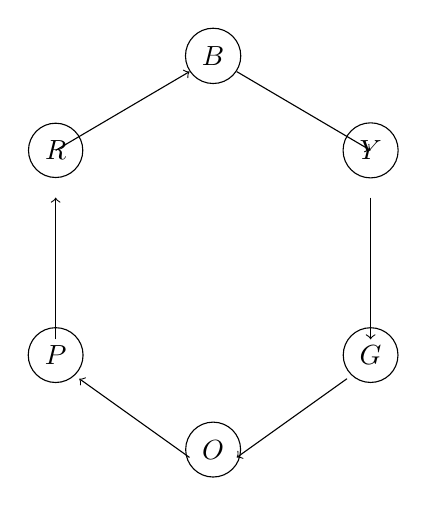
\begin{tikzpicture}[scale=1.0]
\draw[->] (0,2) -- (1.7,3);
\draw[->] (2.3,3) -- (4,2);
\draw[->] (4,1.4) -- (4,-0.4);
\draw[->] (3.7,-0.9) -- (2.3,-1.9);
\draw[->] (1.7,-1.9) -- (0.3,-0.9);
\draw[->] (0,-0.4) -- (0,1.4);

\node[draw,circle] at (0,2) {$R$};
\node[draw,circle] at (2,3.2) {$B$};
\node[draw,circle] at (4,2) {$Y$};
\node[draw,circle] at (4,-0.6) {$G$};
\node[draw,circle] at (2,-1.8) {$O$};
\node[draw,circle] at (0,-0.6) {$P$};
\end{tikzpicture}
\caption{At the moment the deterministic law is being recast as a diagram, the board still carries earlier probability notation on the left. The lecture then turns the textual update rule into a closed six-state cycle.}
\end{figure}

If each step takes the same amount of time and if we do not know the starting point, then sampling the system at an arbitrary instant gives
\begin{equation}
p(R)=p(B)=p(Y)=p(G)=p(O)=p(P)=\frac16.
\end{equation}
The probability comes from equal time spent in each state, not from symmetry of the object.

Susskind strengthens the point by changing the update rule while keeping a single six-step cycle. The order of visitation may change, but as long as each state is visited once per period, the same conclusion follows. The prediction \(1/6\) does not require knowledge of the precise law, only knowledge that the law has this one-cycle structure.

\subsection{Question \& Answer}

\paragraph{Question.} If the system is not symmetric, why can each state still have probability \(1/6\)?

\paragraph{Answer.} Because here probability is not being assigned by geometric symmetry. It is being assigned by the orbit of the deterministic dynamics. If the system moves through six states in a closed cycle and spends the same amount of time in each state, then an observer who does not know the initial moment must assign equal weight to the six time-slots of the cycle. The symmetry relevant here is the symmetry of the orbit in time, not the symmetry of the die in space.

\section{Cycles, Conserved Quantities, And Two Connected Systems}

The next move is the important one. The state space need not consist of a single cycle. It may split into disconnected cycles. For example, imagine one three-cycle
\[
R \to B \to G \to R
\]
and a second three-cycle
\[
P \to Y \to O \to P.
\]
If we know that the system lies on the first cycle, then the probabilities are
\begin{equation}
p(R)=p(B)=p(G)=\frac13,
\qquad
p(P)=p(Y)=p(O)=0.
\end{equation}
If we know it lies on the second cycle, then the reverse statement holds.

But the lecture does not stop there. We may know only that the system starts on the \(+\) cycle with probability \(p_{+}\), and on the \(-\) cycle with probability \(p_{-}\), where
\begin{equation}
p_{+}+p_{-}=1.
\end{equation}
Then the probabilities within each sector are still uniform, but the overall probabilities become
\begin{equation}
p(R)=p(B)=p(G)=\frac{p_{+}}{3},
\qquad
p(P)=p(Y)=p(O)=\frac{p_{-}}{3}.
\end{equation}

This is the first appearance of a conservation law in the lecture. The two cycles may be labeled by a quantity, say \(+1\) on one cycle and \(-1\) on the other. Because the dynamics never carries a state from one cycle into the other, that quantity is conserved. Dynamics tells us how probability is distributed within a sector; it does not tell us the prior probability of being in one sector rather than another. That extra piece of information must come from somewhere else.

This is exactly the point at which Susskind turns from toy models to honest energy. A closed system may be represented as a box with a conserved energy. Two isolated boxes have two separately conserved energies. If the boxes are connected so that energy can flow through a narrow passage, then only the total energy is conserved. The new statistical question is then unavoidable: given the total energy, how is it distributed between the two subsystems?

\begin{figure}[h]
\centering

\includegraphics[width=0.78\textwidth]{lecture_01_figure_03.png}

\begin{tikzpicture}[scale=0.95]
\draw (-4,2.2) -- (-4,-1.4);
\draw (-4,2.2) -- (-0.6,2.2);
\draw (-4,-1.4) .. controls (-2.6,-1.9) and (-1.5,-1.9) .. (-0.6,-1.4);
\draw (-0.6,2.2) -- (-0.6,0.8);
\draw (-0.6,-1.4) -- (-0.6,-0.1);

\draw (0.6,2.0) -- (4.1,2.0);
\draw (4.1,2.0) -- (4.1,-1.6);
\draw (4.1,-1.6) -- (0.6,-1.6);
\draw (0.6,2.0) -- (0.6,0.8);
\draw (0.6,-0.1) -- (0.6,-1.6);

\draw (-0.6,0.8) -- (0.6,0.8);
\draw (-0.6,-0.1) -- (0.6,-0.1);
\end{tikzpicture}
\caption{The lecture's sketch of two connected subsystems. Once the two parts can exchange energy, the statistical question is no longer only which microscopic cycle one occupies, but how a fixed total energy is shared between the parts.}
\end{figure}

One may expect equal subsystems to share energy equally on average, but that is not the whole problem. Statistical mechanics asks for the probability distribution of that sharing. In other words, it asks for the relative weights of sectors defined by conserved quantities.

\section{Good Laws, Bad Laws, And The Minus First Law}

Before proceeding further, the lecture asks a structural question: what sort of laws are even allowed? Susskind's answer is that some laws are bad, not morally bad, but physically inadmissible. The prototype of a bad law is the rule that sends every state to the same state:
\begin{align}
R &\to R, & B &\to R, & Y &\to R, \nonumber\\
G &\to R, & O &\to R, & P &\to R. \label{eq:bad_law}
\end{align}

This law predicts the future trivially well, but it erases the past. If the present state is \(R\), one cannot reconstruct whether the system came from \(B\), \(Y\), \(O\), or anywhere else. Distinctions between states have been destroyed.

Susskind gives this principle a name: the minus first law of physics. Information is not lost. Differences between states propagate forward in time, and if the dynamics is fundamental then in principle one can reconstruct the past from the present. In discrete diagrammatic language, the criterion is simple: a good law is one in which every state has one incoming arrow and one outgoing arrow. That is the discrete analog of reversibility.

In continuum mechanics this becomes Liouville's theorem. A region of occupied phase space may deform and flow, but its phase-space volume is preserved. If the probability density is initially uniform on that occupied region, it remains uniform on the evolved region. The continuous statement is therefore the natural analog of the discrete statement that \(M\) equally probable occupied states remain \(M\) equally probable occupied states under an information-preserving evolution.

\subsection{Question \& Answer}

\paragraph{Question.} Why does friction not really violate conservation of information?

\paragraph{Answer.} Because friction only looks like a bad law when we describe too small a system. If we write, schematically,
\begin{equation}
m\ddot x = -\gamma \dot x,
\end{equation}
then a moving particle exponentially slows down and seems to lose all memory of its initial motion. Taken as a fundamental law for a closed system, this would indeed be disastrous: every particle in a gas would drift toward rest, energy would disappear, and the final state would become simpler rather than more complicated.

But real friction is not a fundamental one-variable law. When an eraser slows down on a table, the information is not annihilated; it is transferred into microscopic degrees of freedom of the eraser, the table, and the surrounding air. In the visible coordinates the motion may contract, but in the full higher-dimensional phase space the distribution spreads into hidden directions. The apparent squeeze is a projection. Liouville volume is preserved once the whole closed system is included.

This is the conceptual role of the friction example in the lecture. It is not there to establish a precise dissipative equation. It is there to show that apparent irreversibility at the macroscopic level is compatible with information preservation at the microscopic level.

\section{The First Law And The Additivity Caveat}

After the minus first law, Susskind jumps over the zeroth law and states the first law in its bare form. It is simply the conservation of energy:
\begin{equation}
\frac{dE}{dt}=0.
\end{equation}
For a closed system, that is the whole statement.

If the system is made of two weakly coupled parts, then the total energy is approximately additive,
\[
E \approx E_1 + E_2,
\]
and therefore
\begin{align}
\frac{dE_1}{dt}+\frac{dE_2}{dt} &= 0, \\
\frac{dE_1}{dt} &= -\frac{dE_2}{dt}.
\end{align}
This is the form that makes the physical meaning transparent: energy lost by one side is gained by the other.

The lecture is careful, however, not to turn this approximation into an exact identity. In a genuinely interacting two-body system there may be potential energy that belongs to neither subsystem separately. The solar system, treated as two Newtonian bodies, does not have an energy equal merely to the kinetic energy of the first body plus the kinetic energy of the second. There is also the energy of interaction between them.

Why then is additive energy so useful in thermodynamics? Because for large systems the interaction energy is often a surface effect while the bulk energy is a volume effect. Divide a large body into blocks: the energy contained in a block scales roughly with its volume, while the interaction across block boundaries scales with surface area. In that regime the interaction term is small enough that the additive approximation is excellent, and the first law can be used in the simple two-subsystem form above.

\section{Entropy As A Measure Of Ignorance}

\subsection{Occupied States And The First Definition}

We now return, as the lecture explicitly does, to unfinished business: entropy. At first Susskind defines it only in a special case. Suppose there are \(N\) possible states altogether, but only \(M\) of them have nonzero probability, and suppose those \(M\) occupied states are all equally probable. Then
\begin{equation}
p_i=\frac{1}{M}
\quad\text{for the occupied states,}
\qquad
p_i=0
\quad\text{for the others.}
\end{equation}
The entropy is then defined by
\begin{equation}
S=\log M.
\end{equation}

This is already enough to capture the central idea. If \(M=N\), every state is equally probable and our ignorance is maximal:
\begin{equation}
S_{\max}=\log N.
\end{equation}
If \(M=1\), the state is known exactly and the entropy is zero.

The lecture emphasizes that \(M\) measures ignorance. The bigger \(M\) is, the less we know. And because a good law merely reshuffles occupied states without changing their number, \(M\) stays fixed under exact microscopic evolution. In that sense entropy is conserved if we can follow the system in complete detail. Entropy increases in practice because we become lazy, coarse, or overwhelmed by the degrees of freedom. The increase reflects loss of knowledge, not loss of microscopic information by the equations themselves.

This is why Susskind insists that entropy, in this lecture, comes before temperature and in a certain sense even before energy. Entropy is being introduced first as a quantitative measure of ignorance.

\subsection{General Probability Distributions}

The special rectangular distribution is too narrow a case. Usually the probabilities are not all equal on the occupied set. The lecture therefore redraws the state space schematically as a horizontal list of states and the probabilities as a graph above it.

\begin{figure}[h]
\centering

\includegraphics[width=0.74\textwidth]{lecture_01_figure_05.png}

\begin{tikzpicture}[scale=0.9]
\draw[->] (-4.2,0) -- (4.4,0);
\draw[->] (-4,0) -- (-4,3.2);
\node at (-4.45,3.0) {$p_i$};

\draw (-3.6,0.1) -- (-3.6,-0.1);
\draw (-3.1,0.1) -- (-3.1,-0.1);
\draw (-2.6,0.1) -- (-2.6,-0.1);
\draw (-2.1,0.1) -- (-2.1,-0.1);
\draw (-1.6,0.1) -- (-1.6,-0.1);
\draw (-1.1,0.1) -- (-1.1,-0.1);
\draw (-0.6,0.1) -- (-0.6,-0.1);
\draw (-0.1,0.1) -- (-0.1,-0.1);
\draw (0.4,0.1) -- (0.4,-0.1);
\draw (0.9,0.1) -- (0.9,-0.1);
\draw (1.4,0.1) -- (1.4,-0.1);
\draw (1.9,0.1) -- (1.9,-0.1);
\draw (2.4,0.1) -- (2.4,-0.1);
\draw (2.9,0.1) -- (2.9,-0.1);
\draw (3.4,0.1) -- (3.4,-0.1);

\draw plot[smooth] coordinates {
(-3.7,0.18) (-3.0,0.25) (-2.4,0.55) (-1.7,1.25)
(-1.0,2.05) (-0.4,2.45) (0.0,2.3) (0.5,1.95)
(1.2,1.35) (1.9,0.8) (2.7,0.42) (3.5,0.18)
};

\draw (-1.9,-0.15) -- (-1.9,-0.45);
\draw (1.8,-0.15) -- (1.8,-0.45);
\draw (-1.9,-0.45) -- (1.8,-0.45);
\node at (-0.05,-0.8) {$M$};
\end{tikzpicture}
\caption{The lecture's schematic probability graph over discrete state labels. The width marked by \(M\) is not a literal count in this smooth picture, but it is the visual cue for the main point: a narrower distribution carries less entropy than a broader one.}
\end{figure}

The definition that handles the general case is
\begin{equation}
S=-\sum_i p_i \log p_i.
\end{equation}
This is, in Susskind's own language, minus the average of \(\log p_i\). The minus sign is necessary because probabilities are smaller than \(1\), and therefore their logarithms are negative.

The lecture immediately checks that this new definition reproduces the old one when it should. If \(p_i=1/M\) on the occupied set and \(p_i=0\) elsewhere, then the unoccupied states contribute nothing because
\begin{equation}
\lim_{p\to 0^+} p\log p = 0.
\end{equation}
For the occupied states we obtain
\begin{align}
S
&= - \sum_{\text{occupied }i} \frac{1}{M}\log\!\left(\frac{1}{M}\right) \\
&= - M \left[\frac{1}{M}\log\!\left(\frac{1}{M}\right)\right] \\
&= -\log\!\left(\frac{1}{M}\right) \\
&= \log M.
\end{align}
So the general formula is consistent with the original \(S=\log M\).

The lecture then interprets the graph qualitatively. If the distribution is narrow, only a relatively small collection of states matters appreciably, and the entropy is small. If the distribution is broad, many states carry significant weight, and the entropy is larger. The later lecture frame below reinforces exactly this point by drawing attention to the width \(M\).

\begin{figure}[h]
\centering

\includegraphics[width=0.72\textwidth]{lecture_01_figure_06.png}
\caption{A later frame of the same graph. The lecturer's gesture emphasizes that what matters qualitatively is the spread of the distribution: narrower means smaller entropy, broader means larger entropy.}
\end{figure}

\subsection{Coins As Explicit Examples}

The lecture now turns back to coins, because they let us calculate with complete clarity. To keep notation consistent, let \(n\) denote the number of coins, and let \(N\) denote the total number of states of the \(n\)-coin system. Then
\begin{equation}
N=2^n.
\end{equation}

If we know nothing at all, every one of the \(2^n\) states is equally probable. Therefore
\begin{equation}
S=\log(2^n)=n\log 2.
\end{equation}
This is maximal entropy for the \(n\)-coin system.

If instead we know the state completely, then only one state has nonzero probability. In that case \(M=1\), and
\begin{equation}
S=0.
\end{equation}
Perfect knowledge corresponds to zero entropy.

A more interesting case is this: all coins are heads except for exactly one tail, but we do not know which coin is tails. Then there are exactly \(n\) states with nonzero probability, all equally weighted, and so
\begin{equation}
S=\log n.
\end{equation}
This is an important example in the lecture because it shows that entropy need not be an integer multiple of \(\log 2\) when we use natural logarithms.

Susskind also pauses to discuss the base of the logarithm. In these notes, as in the lecture, \(\log\) means the natural logarithm. In information theory one often uses base \(2\), in which case the entropy of a completely unknown single coin is \(1\) bit. The choice of base changes only an overall multiplicative factor. The content of the formula does not change.

\subsection{Continuous Phase Space}

The lecture then enlarges the discrete picture to ordinary mechanics. A classical state is no longer a discrete label but a point in phase space, specified by coordinates and momenta. We may think schematically of the state as a point in \((x,p)\)-space, with the understanding that a real many-particle system has vastly more dimensions.

Suppose first that the probability distribution is uniform on some occupied blob of phase space and zero outside. Then the continuous analog of counting occupied states is measuring the volume of that occupied region. The entropy is defined by
\begin{equation}
S=\log V_{\Gamma},
\end{equation}
where \(V_{\Gamma}\) is the phase-space volume of the occupied blob.

For a general probability density \(P\) on phase space we replace sums by integrals. The normalization condition becomes
\begin{equation}
\int d\Gamma\, P = 1,
\end{equation}
and the entropy becomes
\begin{equation}
S=-\int d\Gamma\, P\log P.
\end{equation}

This is the continuous analog of the discrete formula, and conceptually it does the same job. In the first instance it measures the logarithm of the volume of the probability blob; more generally it measures, in a weighted way, how spread out the probability distribution is.

The lecture is very explicit about the interpretation. Entropy is associated with a probability distribution on the space of possible states. It is not like energy or momentum, which belong to a single microscopic state of the system. Entropy depends both on the system and on our state of knowledge of that system.

\subsection{Correlation And Additivity}

The final discussion of the lecture sharpens this interpretation by introducing correlation. If we know nothing about a collection of coins and then measure one of them, we learn nothing about the others. That is the uncorrelated case.

But if we know that exactly one coin among \(n\) is tails, then measuring one coin changes what we know about the rest. If the measured coin is tails, all the others are surely heads. If the measured coin is heads, then the probability that any one of the remaining coins is the tail becomes
\begin{equation}
p(\text{tail on a given remaining coin}\mid \text{measured head})=\frac{1}{n-1}.
\end{equation}
This is correlation in Susskind's sense: measuring one part modifies the probability distribution of another part.

Entropy is additive when there is no correlation. For uncorrelated subsystems, the total entropy is the sum of the entropies of the parts. The lecture ends by asking the audience to imagine more complicated correlated distributions, for example chains of coins in which one measurement biases the probabilities of neighboring coins, and to compute the corresponding entropy. The point is not to finish the calculation on the spot. The point is to see that entropy is really tracking organized ignorance, and organized ignorance is altered by correlation.

The audience then raises the relation to information theory. Susskind's answer is that Boltzmann's and Shannon's entropies are the same formula up to the base of the logarithm and a convention about the overall sign. What is called entropy here is therefore a measure of lack of information. It is not the Heisenberg uncertainty principle. It concerns probabilistic ignorance described by a distribution over states, not the distinct issue of quantum uncertainty in a pure state.

\section{Summary}

The first lecture lays the foundation in a very definite order. Statistical mechanics is introduced as a deep and general part of physics; then probability is reviewed as the right language for incomplete knowledge; then deterministic update laws are used to show how probabilities can emerge from ignorance of the starting point; then conservation laws and the conservation of information are brought in to constrain what sort of dynamics are allowed.

Only after that groundwork does the lecture state the first law and turn fully to entropy. Entropy begins as \(\log M\), the logarithm of the number of equally probable occupied states, and then broadens to
\[
S=-\sum_i p_i\log p_i
\]
and, in phase space,
\[
S=-\int d\Gamma\,P\log P.
\]
In every form it measures ignorance encoded in a probability distribution. That is the central lesson of this first meeting with statistical mechanics. Temperature and thermal equilibrium are deferred to the next lecture; entropy has been put in place first.